% !TeX root = ../../Skript.tex
\cohead{\Large\textbf{Nullstellen}}
\fakesubsection{Nullstellen}
In der Mathematik unterscheidet man grundsätzlich zwischen Stellen und Punkten. Stellen sind x-Werte während Punkte einen x-Wert und einen y-Wert haben. Die Nullstellen (abgekürzt NST) sind die Stellen, an denen die Funktion die x-Achse schneidet.Oder anders ausgedrückt, die NST sind die Stellen, an denen der Funktionswert bzw. y-Wert Null ist:
\begin{tcolorbox}
	\centering
	\textcolor{loestc}{\(f(x)=0\)}
\end{tcolorbox}

\textbf{Beispiel:}

\adjustbox{valign=t}{\begin{minipage}{0.55\textwidth}
	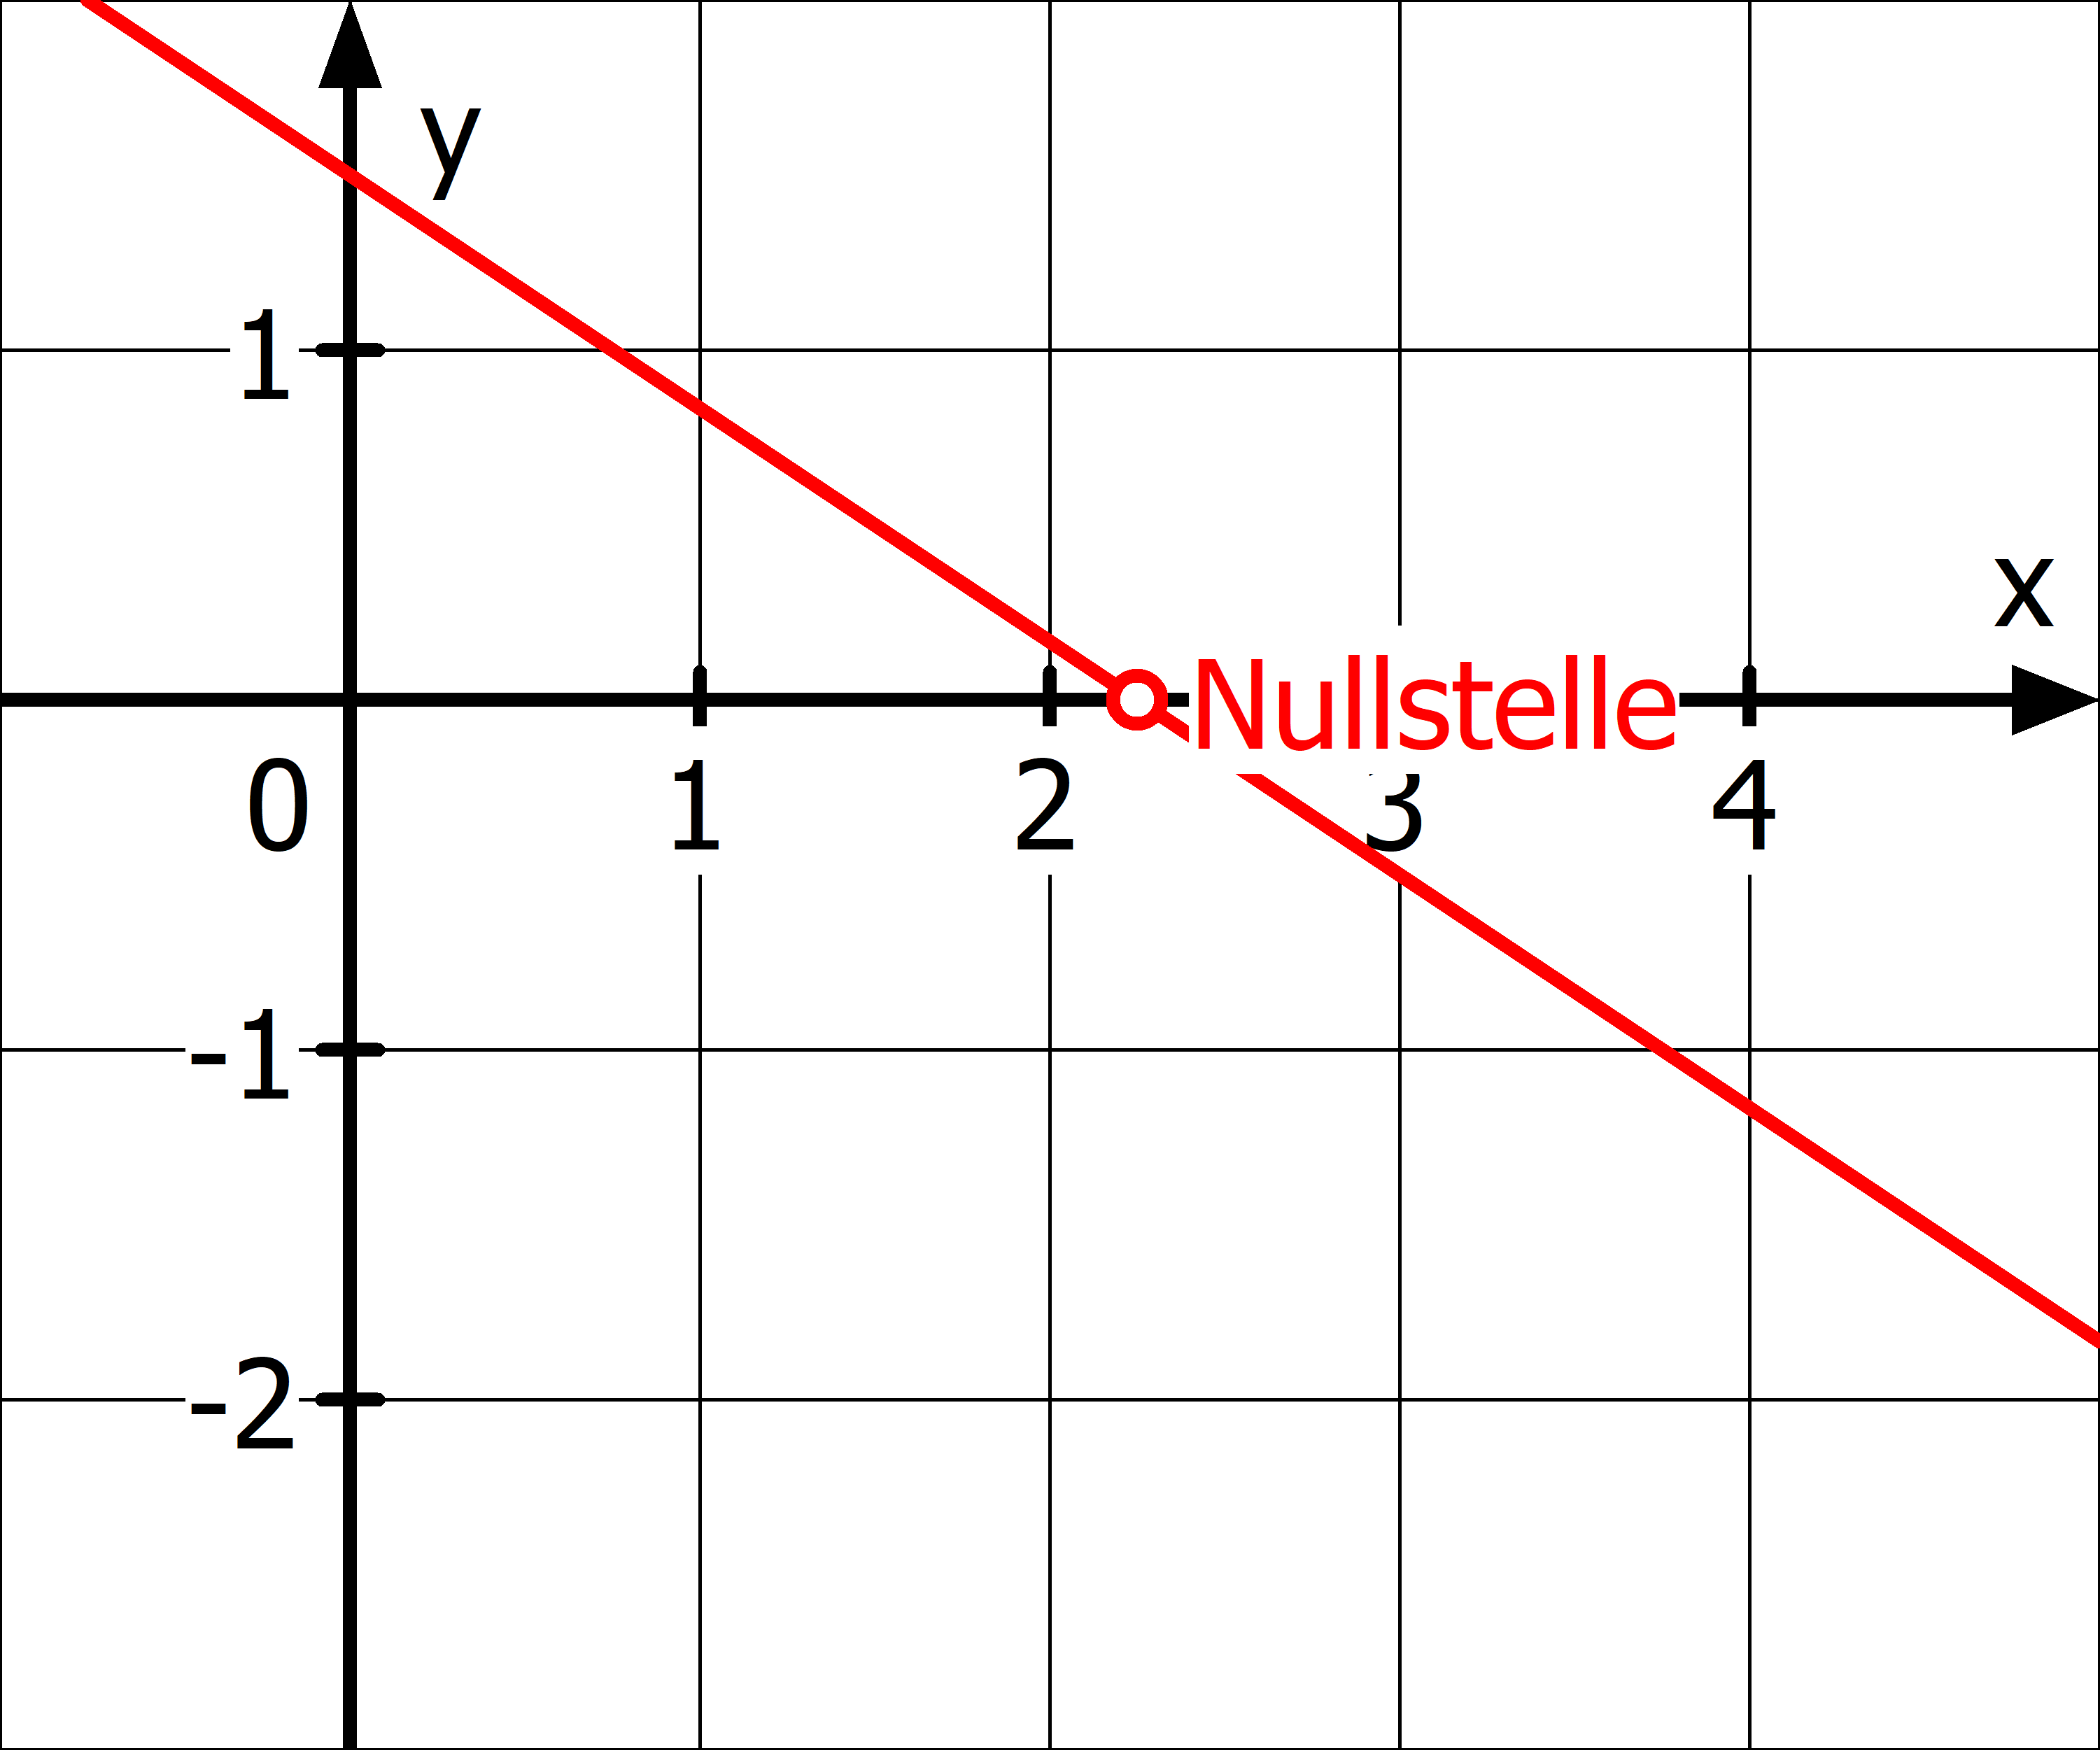
\includegraphics[width=0.95\textwidth]{\linFkt/pics/nullstelle.png}
\end{minipage}}%
\adjustbox{valign=t}{\begin{minipage}{0.45\textwidth}
	Gegeben ist die Funktion \(f(x)=-\tfrac{2}{3}x+\tfrac{3}{2}\).
	Im Schaubild kann man die Nullstelle ungefähr ablesen: \(x_0\approx 2,2\).

	Um den exakten Wert zu erhalten, muss man folgende Gleichung lösen:
	\begin{align*}
		\textcolor{loes}{f(x)}&\textcolor{loes}{=0}\\
		\textcolor{loes}{-\tfrac{2}{3}x+\tfrac{3}{2}}&\textcolor{loes}{=0\ \vert-\dfrac{3}{2}}\\
		\textcolor{loes}{-\tfrac{2}{3}x}&\textcolor{loes}{=-\tfrac{3}{2}\ \vert\cdot\left(-\tfrac{3}{2}\right)}\\
		\textcolor{loes}{\Rightarrow x_0}&\textcolor{loes}{=\tfrac{9}{4}=2,25}
	\end{align*}
\end{minipage}}%

\begin{Exercise}[title={Bestimme die Nullstellen}, label=nullstellenA1]

	\begin{minipage}{0.5\textwidth}
		\begin{enumerate}[label=\alph*)]
			\item \(f_1(x)=3x-9\)
			\item \(f_2(x)=-2x-10\)
			\item \(f_3(x)=\frac{2}{3}x+4\)
			\item \(f_4(x)=-\frac{3}{4}x+12\)
			\item \(f_5(x)=\frac{5}{2}x+\frac{10}{3}\)
		\end{enumerate}
	\end{minipage}%
	\begin{minipage}{0.5\textwidth}
		\begin{enumerate}[label=\alph*)]
			\setcounter{enumi}{5}
			\item \(f_6(x)=-0,5x-3,2\)
			\item \(f_7(x)=-8+2x\)
			\item \(f_8(x)=\frac{5}{7}-\frac{15}{14}x\)
			\item \(f_9(x)=3(2x-5)\)
			\item \(f_{10}(x)=\frac{1}{3}\left(6x-5\right)+\frac{5}{6}\)
		\end{enumerate}
	\end{minipage}%
\end{Exercise}\vspace{0,5cm}
\begin{Answer}[ref=nullstellenA1]

	\begin{minipage}{0.5\textwidth}
		\begin{enumerate}[label=\alph*)]
			\item \(x_0=3\)
			\item \(x_0=-5\)
			\item \(x_0=-6\)
			\item \(x_0=16\)
			\item \(x_0=-\frac{4}{3}\)
		\end{enumerate}
	\end{minipage}%
	\begin{minipage}{0.5\textwidth}
		\begin{enumerate}[label=\alph*)]
			\setcounter{enumi}{5}
			\item \(x_0=-6,4\)
			\item \(x_0=4\)
			\item \(x_0=\frac{2}{3}\)
			\item \(x_0=\frac{5}{2}\)
			\item \(x_0=\frac{5}{12}\)
		\end{enumerate}
	\end{minipage}%
\end{Answer}